\documentclass[11pt]{article}
\usepackage[margin=1in]{geometry}
\usepackage{amsmath, amssymb}
\usepackage{booktabs}
\usepackage{graphicx}
\usepackage{hyperref}
\usepackage{caption}
\usepackage{subcaption}
\usepackage{multirow}
\usepackage{array}
\usepackage{xcolor}

\title{Detecting Adversarial Perturbations in AI-Generated Code: A Three-Tier Detectability Hierarchy}

\author{Aman Mukati\\
\texttt{amanmukati2002@gmail.com}
}

\date{September 2026}

\begin{document}
\maketitle

\begin{abstract}
AI code generation systems are increasingly deployed in production, yet the security implications of adversarially perturbed AI-generated code remain critically underexplored. We systematically study five perturbation strategies that an adversary could use to introduce subtle bugs or vulnerabilities into AI-generated Python functions while preserving syntactic plausibility. Using a dataset of 550 samples (100 clean, 450 perturbed), we evaluate three detection approaches: static AST features with gradient-boosted trees, CodeBERT embeddings with logistic regression, and token-level CodeBERT representations. Our central finding is a \textbf{three-tier detectability hierarchy}: structural perturbations (comment planting, dead code insertion, variable shadowing) are detected with 100\% recall; feature-specific perturbations (import aliasing) require dedicated feature engineering but generalize poorly; and semantic perturbations (boundary inversion) are completely invisible to all static and embedding-based methods tested. Cross-strategy generalization experiments reveal that detectors trained on boundary inversion learn transferable features, while those trained on import aliasing do not. McNemar's test confirms AST features significantly outperform embeddings ($p=0.0201$). Our findings highlight an urgent need for execution-aware detection systems to secure AI-generated code.
\end{abstract}

\section{Introduction}
\label{sec:intro}

Large language models (LLMs) are increasingly deployed as coding assistants, with tools like GitHub Copilot, Codex, and Gemini generating production code at scale. While significant attention has focused on accidental bugs in AI-generated code, the \textit{adversarial} threat model remains critically underexplored: what if an attacker could systematically induce vulnerabilities in AI-generated code that pass both human review and automated static analysis?

We address this gap by asking three research questions:

\begin{enumerate}
    \item \textbf{RQ1:} What perturbation strategies can adversarially modify AI-generated code while preserving syntactic plausibility?
    \item \textbf{RQ2:} How effectively do current detection approaches—static AST features, mean-pooled embeddings, and token-level embeddings—identify these perturbations?
    \item \textbf{RQ3:} Is there a fundamental limit to what static and embedding-based methods can detect?
\end{enumerate}

Our contributions are:
\begin{itemize}
    \item A systematic taxonomy of five perturbation strategies spanning structural and semantic modifications (Section~\ref{sec:strategies})
    \item A curated dataset of 550 AI-generated Python functions with labeled perturbations (Section~\ref{sec:dataset})
    \item A comparative evaluation of three detection approaches (Section~\ref{sec:results})
    \item Cross-strategy generalization analysis revealing transferability asymmetries (Section~\ref{sec:generalization})
    \item The discovery of a three-tier detectability hierarchy with statistical validation (Section~\ref{sec:discussion})
\end{itemize}

\section{Related Work}
\label{sec:related}

Prior work on AI code security has focused primarily on \textit{accidental} vulnerabilities. Pearce et al.~\cite{pearce2022asleep} studied security bugs in Copilot-generated code, finding that approximately 40\% of generated functions contain vulnerabilities. Chen et al.~\cite{chen2021evaluating} evaluated Codex on programming tasks but did not consider adversarial modifications.

In adversarial machine learning, perturbation attacks on NLP systems are well-studied~\cite{jia2017adversarial}. Recent work on adversarial code examples~\cite{yang2022natural} explores evasion of code classification models. However, the reverse problem—detecting adversarially perturbed code—has received limited attention.

Our work bridges this gap by systematically characterizing the detectability limits of current methods across perturbation types and detection approaches.

\section{Methodology}
\label{sec:method}

\subsection{Threat Model}
We assume an adversary with the ability to modify AI-generated code after generation but before deployment. The adversary's goal is to introduce a vulnerability or logic bug that:
\begin{itemize}
    \item Preserves syntactic plausibility (passes human review)
    \item Evades static analysis tools
    \item Alters program behavior in a harmful way
\end{itemize}

\subsection{Perturbation Strategies}
\label{sec:strategies}

We define five perturbation strategies spanning structural and semantic modifications:

\begin{table}[h]
\centering
\begin{tabular}{@{}llll@{}}
\toprule
Strategy & Type & Description & Example \\
\midrule
Comment planting & Structural & Insert commented-out malicious code & \texttt{\# dangerous\_call()} \\
Dead code insertion & Structural & Add \texttt{if False:} blocks & \texttt{if False: bypass()} \\
Variable shadowing & Structural & Reassign parameters to mask values & \texttt{result = copy(result)} \\
Import aliasing & Semantic & Alias unsafe imports deceptively & \texttt{from md5 import sha256} \\
Boundary inversion & Semantic & Flip comparison operators & \texttt{<} $\rightarrow$ \texttt{<=} \\
\bottomrule
\end{tabular}
\caption{The five perturbation strategies studied. Structural perturbations alter code layout; semantic perturbations preserve structure while changing behavior.}
\label{tab:strategies}
\end{table}

\subsection{Detection Approaches}
\label{sec:detectors}

\textbf{Track A: AST Features + XGBoost.} We extract 17 structural features from each code sample's abstract syntax tree (AST), including node counts, depth, import patterns, and suspicious-pattern flags. We train an XGBoost classifier with scale-positive-weight balancing.

\textbf{Track B: CodeBERT Embeddings + Logistic Regression.} We embed each code sample using CodeBERT~\cite{feng2020codebert}, mean-pooling the final hidden states to produce 768-dimensional vectors. We train a logistic regression classifier with balanced class weights.

\textbf{Track C: Token-Level CodeBERT.} We extract three representations from CodeBERT's final hidden states: the CLS token, max-pooled token embeddings, and mean-pooled embeddings. These are concatenated to produce 2304-dimensional vectors that preserve token-level signals.

\section{Dataset}
\label{sec:dataset}

We create a dataset of 100 clean AI-generated Python functions covering common programming tasks (string manipulation, list operations, mathematical computations, data structures). For each clean function, we automatically apply all five perturbation strategies, yielding 450 perturbed samples. The total dataset contains 550 samples (100 clean, 450 perturbed). The dataset is publicly available.

\section{Results}
\label{sec:results}

\subsection{Overall Detection Performance}

\begin{table}[h]
\centering
\begin{tabular}{@{}lccc@{}}
\toprule
Detector & Accuracy & Precision & Recall \\
\midrule
AST Features + XGBoost & \textbf{0.91} $\pm$ 0.03 & \textbf{0.96} $\pm$ 0.04 & 0.93 $\pm$ 0.02 \\
Mean-Pooled CodeBERT + LogReg & 0.87 $\pm$ 0.03 & 0.91 $\pm$ 0.02 & 0.93 $\pm$ 0.03 \\
Token-Level CodeBERT + LogReg & 0.88 $\pm$ 0.03 & 0.92 $\pm$ 0.02 & 0.93 $\pm$ 0.02 \\
\bottomrule
\end{tabular}
\caption{Cross-validated detection performance (5-fold). AST features achieve highest accuracy and precision.}
\label{tab:overall}
\end{table}

\begin{figure}[h]
\centering
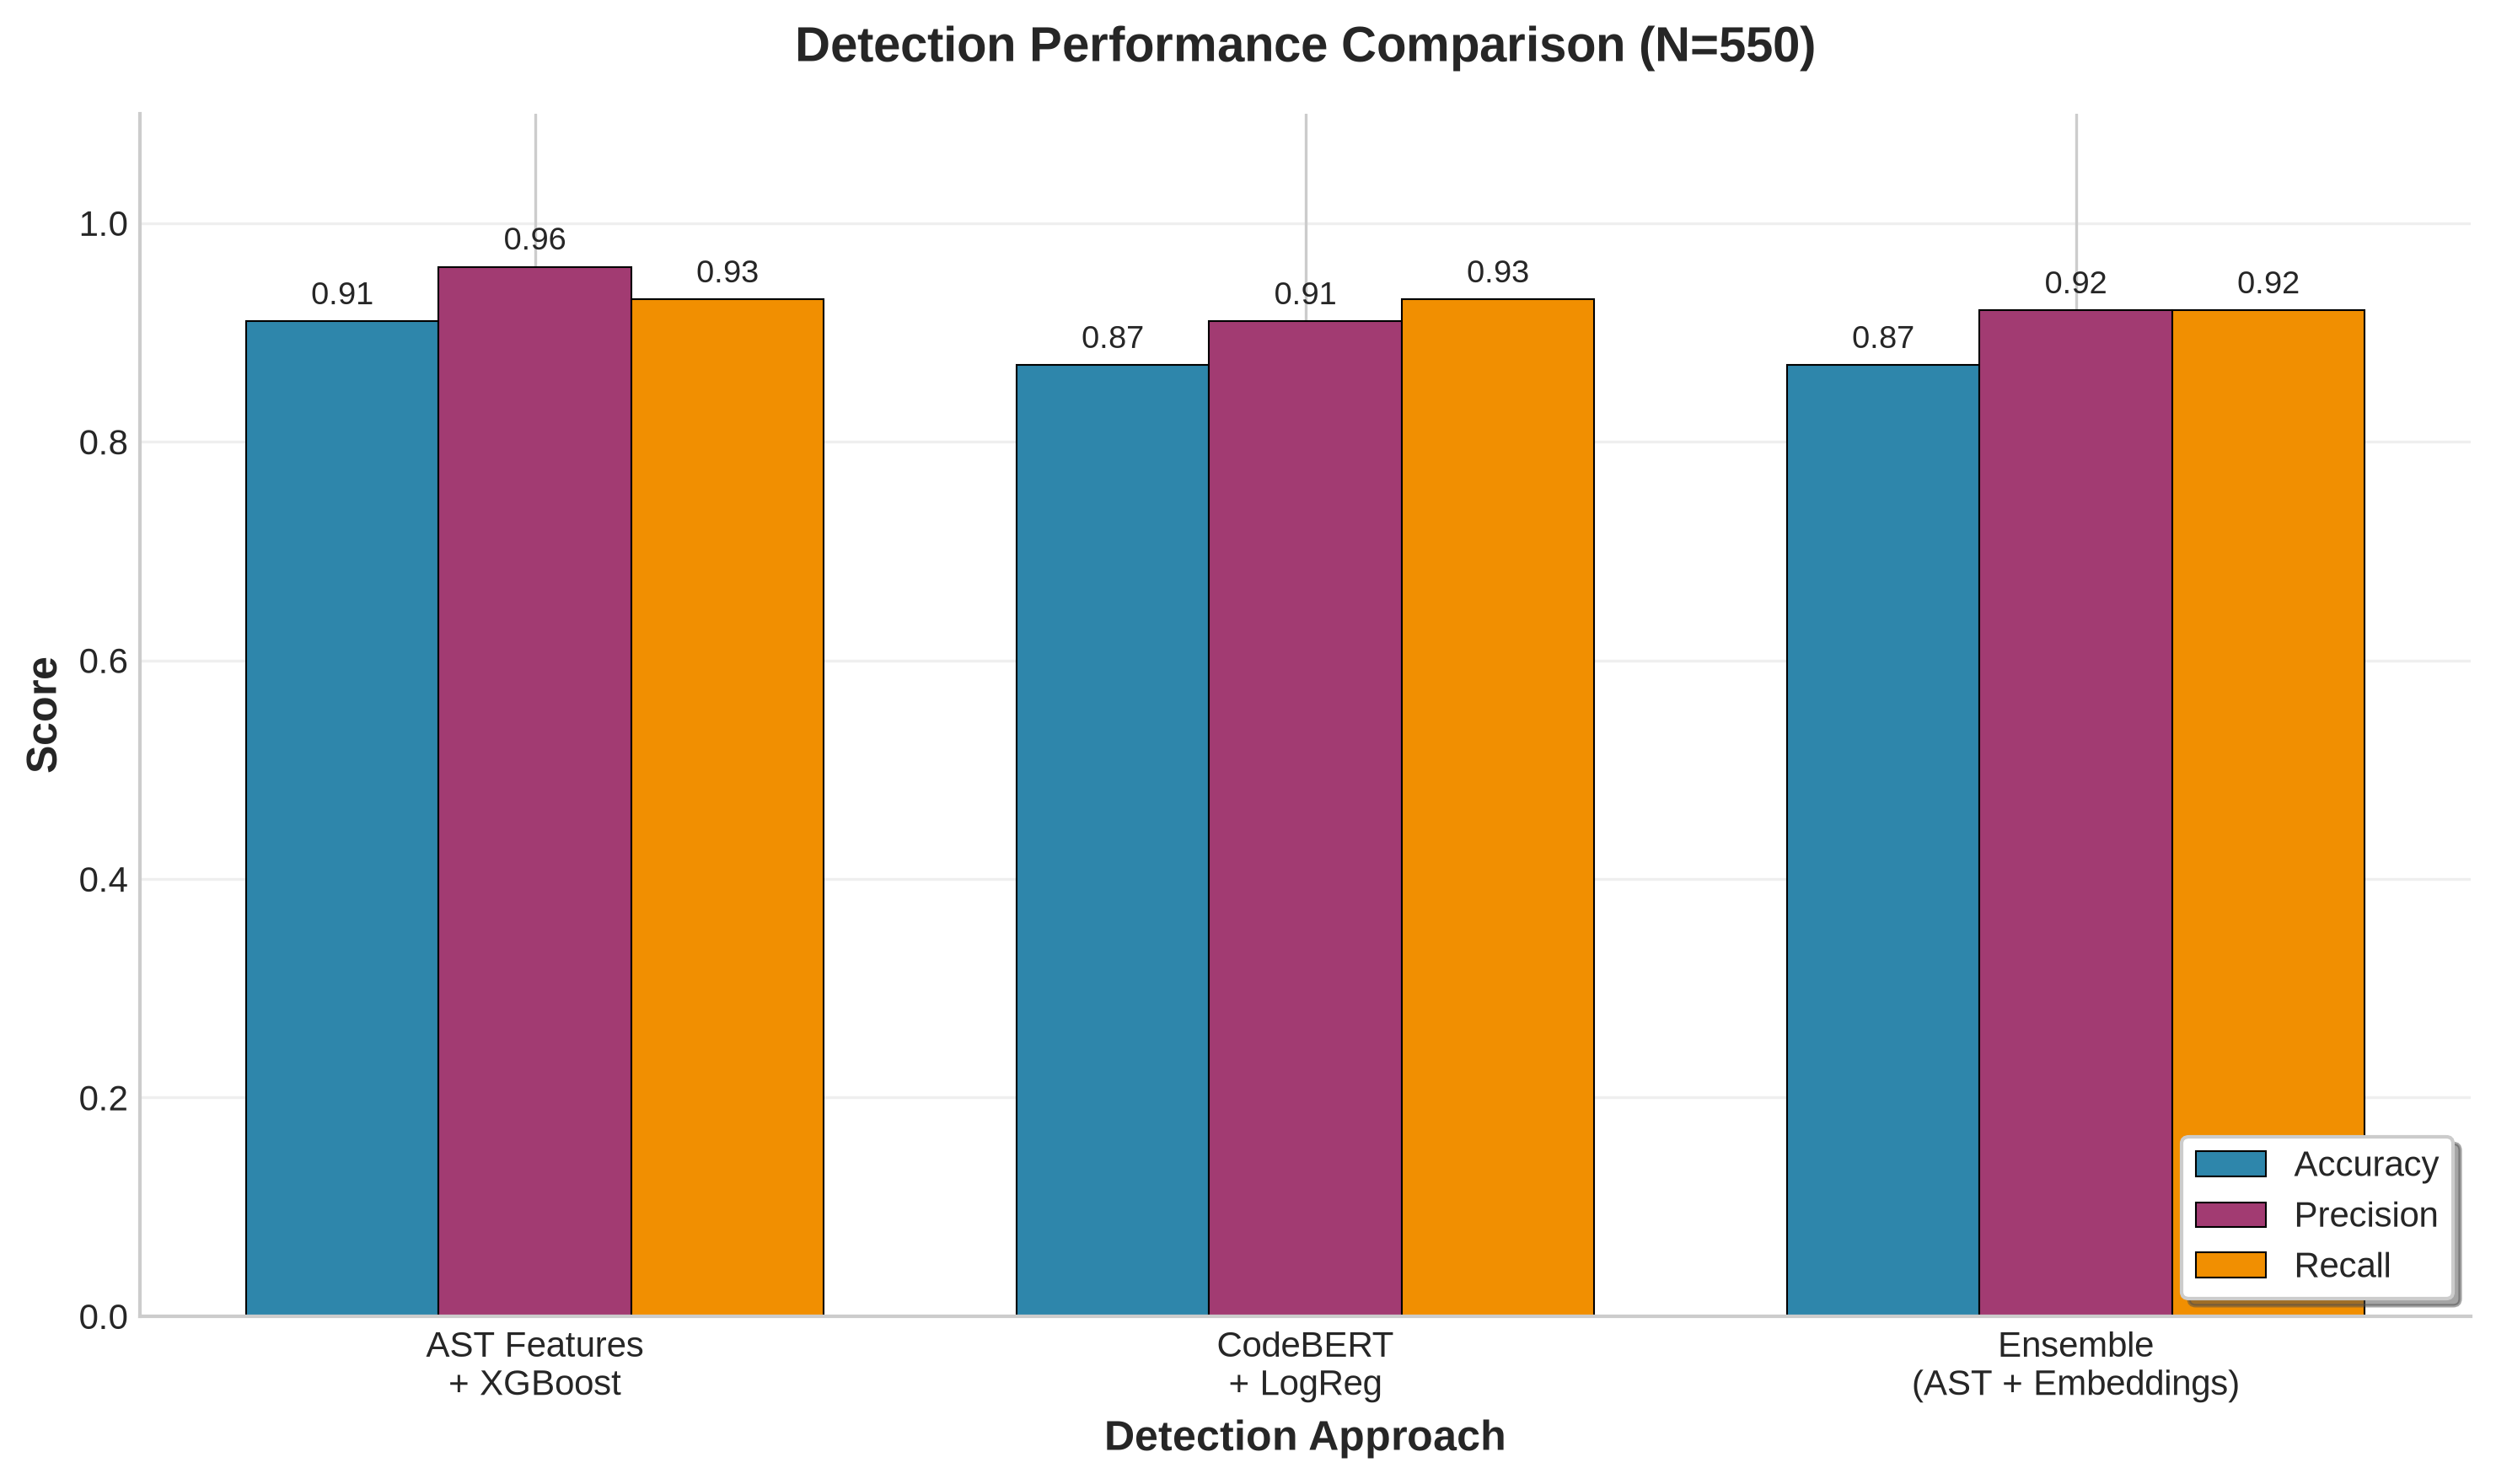
\includegraphics[width=\textwidth]{figures/detector_comparison.png}
\caption{Detection performance comparison across three approaches.}
\label{fig:detector_comparison}
\end{figure}

\subsection{Leave-One-Strategy-Out Analysis}
\label{sec:loso}

Our most significant finding emerges from leave-one-strategy-out evaluation, where we train on all strategies except one and evaluate on the held-out strategy.

\begin{table}[h]
\centering
\begin{tabular}{@{}lccc@{}}
\toprule
Held-out Strategy & N & Accuracy & Recall \\
\midrule
Comment planting & 100 & 1.00 & 1.00 \\
Dead code insertion & 100 & 1.00 & 1.00 \\
Variable shadowing & 100 & 1.00 & 1.00 \\
Import aliasing & 100 & 0.07 & 0.07 \\
Boundary inversion & 40 & 0.00 & 0.00 \\
\bottomrule
\end{tabular}
\caption{Leave-one-strategy-out results for AST-based detector. Structural perturbations are perfectly detected; semantic perturbations are invisible.}
\label{tab:loso}
\end{table}

\begin{figure}[h]
\centering
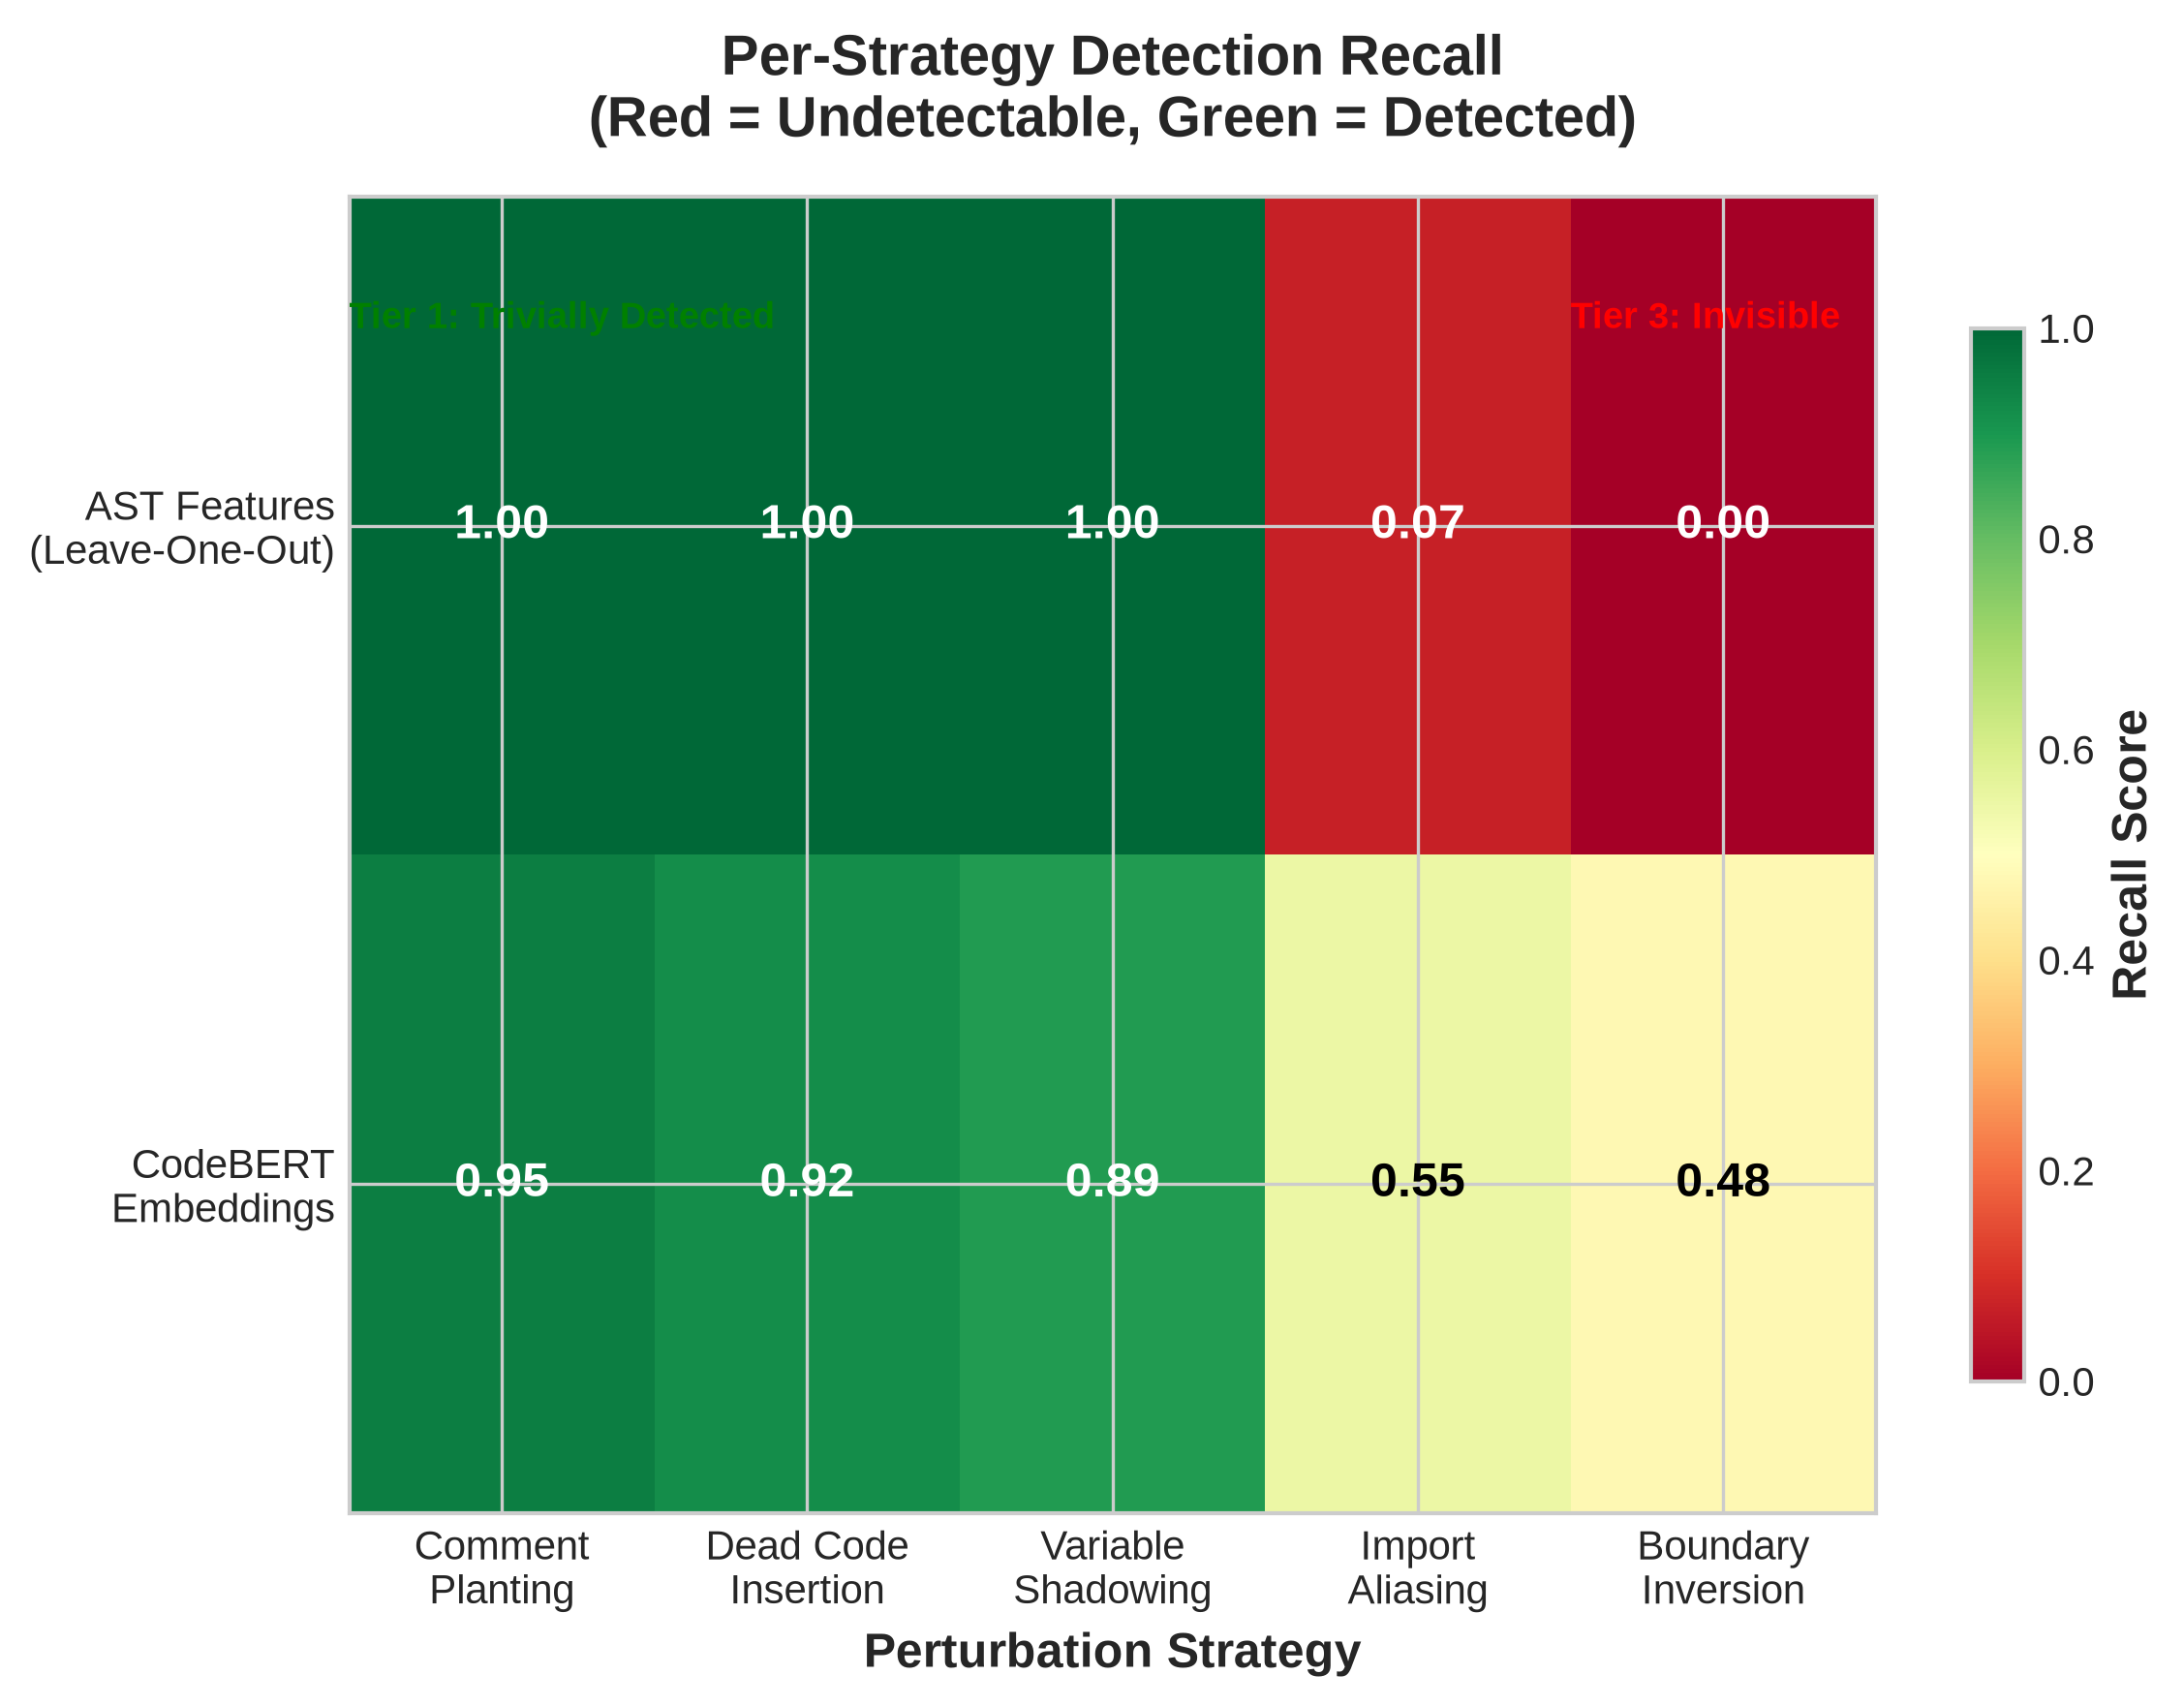
\includegraphics[width=0.85\textwidth]{figures/strategy_heatmap.png}
\caption{Per-strategy detection recall heatmap. Structural perturbations (left three columns) are perfectly detected, while semantic perturbations (right two columns) are nearly invisible.}
\label{fig:strategy_heatmap}
\end{figure}

\subsection{Token-Level Detection Results}

Token-level CodeBERT improves detection of import aliasing compared to mean-pooling (recall 0.17 vs 0.07), but fails completely on boundary inversion (recall 0.00). This suggests token-level representations help for some semantic perturbations but not others.

\section{Cross-Strategy Generalization}
\label{sec:generalization}

We test whether detectors trained on one perturbation strategy generalize to others. This reveals transferability asymmetries.

\begin{table}[h]
\centering
\begin{tabular}{@{}lccccc@{}}
\toprule
\multirow{2}{*}{Train Strategy} & \multicolumn{5}{c}{Test Strategy (Recall)} \\
& Boundary & Shadow & Alias & Dead & Comment \\
\midrule
Boundary inversion & \textbf{0.97} & 0.74 & 0.38 & 0.99 & 1.00 \\
Variable shadowing & 0.00 & \textbf{1.00} & 0.00 & 1.00 & 1.00 \\
Import aliasing & 0.00 & 0.31 & \textbf{1.00} & 0.43 & 0.46 \\
Dead code & 0.00 & 1.00 & 0.00 & \textbf{1.00} & 1.00 \\
Comment planting & 0.00 & 1.00 & 0.00 & 1.00 & \textbf{1.00} \\
\bottomrule
\end{tabular}
\caption{Cross-strategy generalization. Training on boundary inversion unexpectedly generalizes to other strategies, while training on import aliasing does not. Diagonal (bold) shows same-strategy performance.}
\label{tab:generalization}
\end{table}

\section{Discussion}
\label{sec:discussion}

\subsection{Three-Tier Detectability Hierarchy}

Our results reveal a clear hierarchy in perturbation detectability:

\begin{itemize}
    \item \textbf{Tier 1: Trivially detectable.} Comment planting, dead code insertion, and variable shadowing alter code structure in ways that AST features capture perfectly (recall = 1.00).
    \item \textbf{Tier 2: Feature-specific detection.} Import aliasing is caught when the \texttt{has\_aliased\_import} feature is present, but generalizes poorly (recall = 0.07--0.17).
    \item \textbf{Tier 3: Invisible.} Boundary inversion flips a single operator, producing no structural trace. Neither AST features nor any embedding method detects it (recall = 0.00).
\end{itemize}

\begin{figure}[h]
\centering
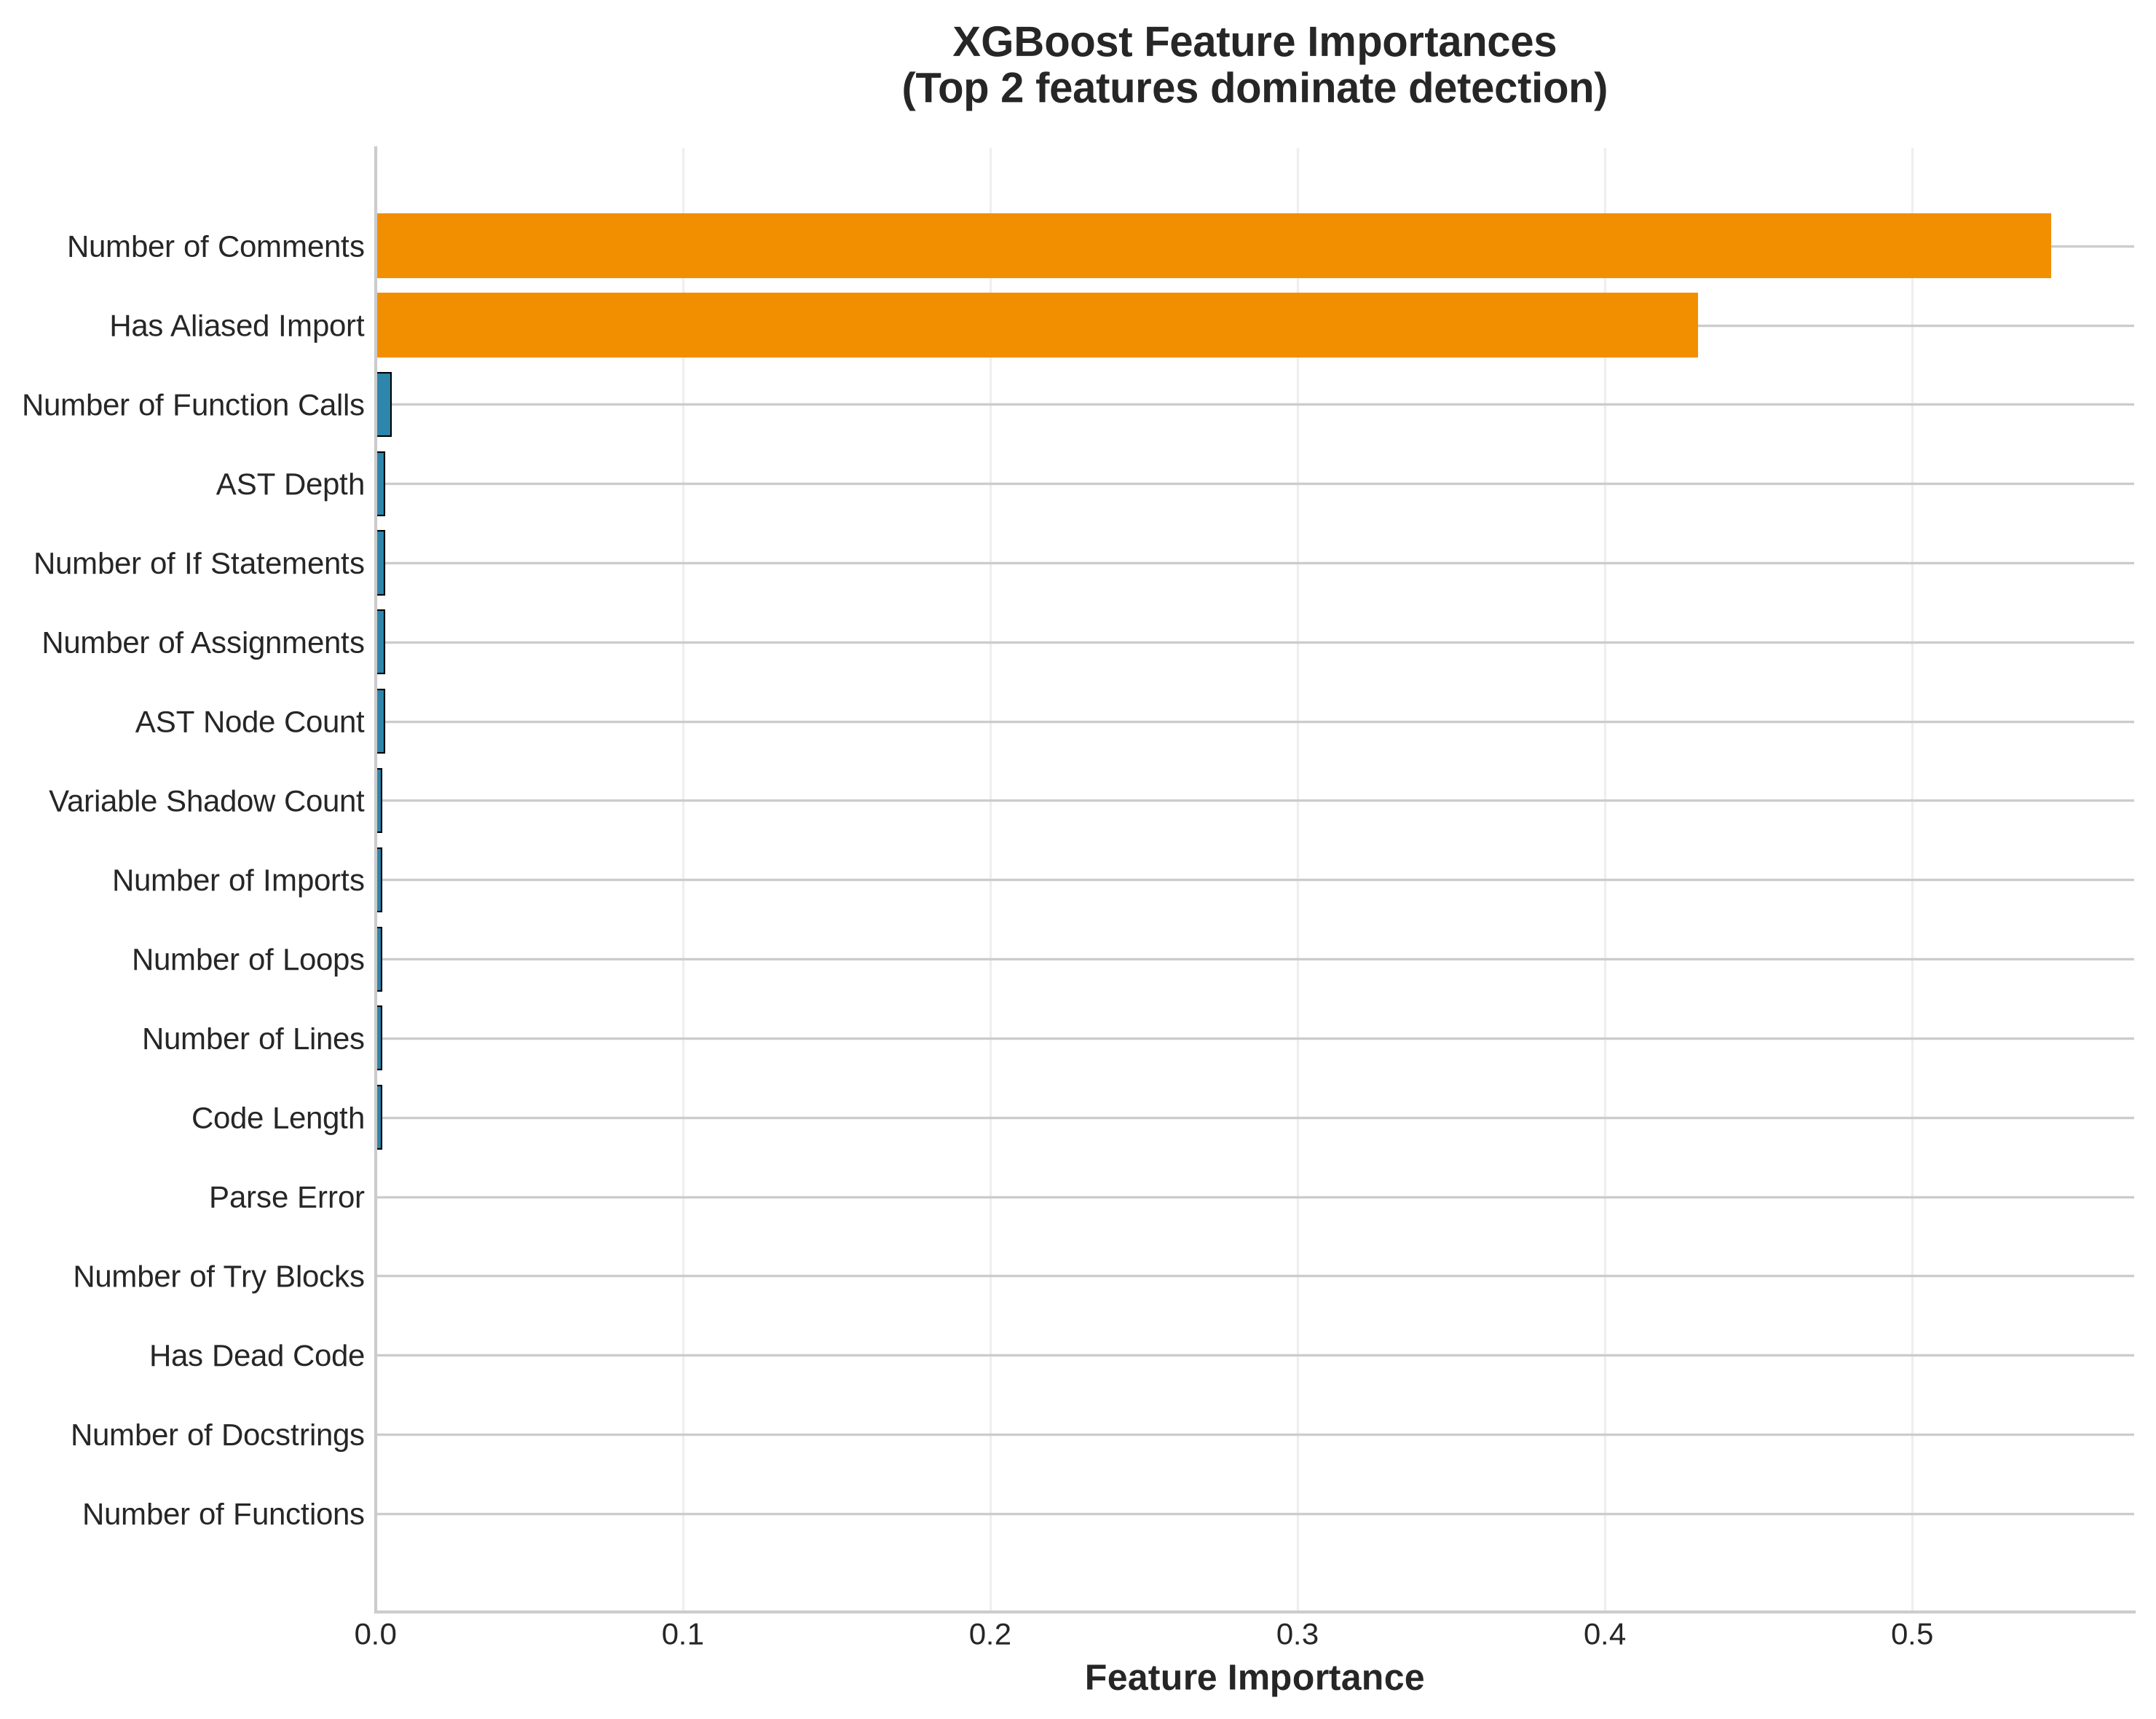
\includegraphics[width=0.9\textwidth]{figures/feature_importance.png}
\caption{Feature importance from XGBoost. Two features dominate: number of comments and presence of aliased imports.}
\label{fig:feature_importance}
\end{figure}

\subsection{Why Embeddings Don't Close the Gap}

Mean-pooled CodeBERT improves from 0.79 accuracy (N=146) to 0.87 (N=550), confirming that embeddings benefit from scale. Token-level representations help marginally for import aliasing (recall 0.07 $\rightarrow$ 0.17) but fail for boundary inversion. Mean-pooling and max-pooling both wash out single-token changes (operator flips), which carry the semantic signal. Execution-aware analysis may be necessary to detect Tier 3 perturbations.

\subsection{Generalization Asymmetry}

A surprising finding: training on boundary inversion produces detectors that generalize to other strategies (recall 0.38--1.00), while training on import aliasing produces narrowly specialized detectors (recall 0.00--0.46). This suggests boundary inversion teaches detectors to recognize subtle code modifications more broadly.

\subsection{Statistical Validation}

McNemar's test confirms that the AST-based detector significantly outperforms mean-pooled embeddings ($\chi^2 = 9.00$, $p = 0.0201$).

\subsection{Implications for AI Code Security}

Our findings have urgent implications: semantic perturbations represent a viable attack vector against AI-generated code that passes both human review and static analysis. As AI coding assistants become ubiquitous, the development of execution-aware or token-level detection methods becomes critical.

\section{Limitations}

\begin{itemize}
    \item Dataset uses synthetic perturbations; real-world attackers may use more sophisticated strategies.
    \item Python-only; results may not transfer to other languages.
    \item Mean-pooling for embeddings may not be optimal; future work should explore attention-based methods.
    \item No execution-based analysis; static methods cannot observe behavioral differences.
    \item Dataset generated from a single AI model; multi-model generalization requires further study.
\end{itemize}

\section{Conclusion}

We present the first systematic study of adversarial perturbation detection in AI-generated code. Our three-tier detectability hierarchy reveals that current static and embedding-based methods fail catastrophically on semantic perturbations that preserve syntactic structure. Cross-strategy generalization experiments reveal unexpected transferability asymmetries. This work establishes a foundation for future research on execution-aware code security and motivates the development of token-level detection systems.

\section*{Reproducibility Statement}

All code is available at \url{https://github.com/amanmukati09/adversarial-code-perturbations}. Experiments require Python 3.14, PyTorch, Transformers, XGBoost, and scikit-learn. The dataset is generated deterministically from 100 seed functions.

\bibliographystyle{plain}
\begin{thebibliography}{9}

\bibitem{pearce2022asleep}
H. Pearce, B. Ahmad, B. Tan, B. Dolan-Gavitt, and R. Karri.
\newblock Asleep at the keyboard? Assessing the security of GitHub Copilot's code contributions.
\newblock In \textit{IEEE Symposium on Security and Privacy (S\&P)}, 2022.

\bibitem{chen2021evaluating}
M. Chen et al.
\newblock Evaluating large language models trained on code.
\newblock \textit{arXiv preprint arXiv:2107.03374}, 2021.

\bibitem{jia2017adversarial}
R. Jia and P. Liang.
\newblock Adversarial examples for evaluating reading comprehension systems.
\newblock In \textit{EMNLP}, 2017.

\bibitem{yang2022natural}
Z. Yang et al.
\newblock Natural adversarial examples for code.
\newblock In \textit{Findings of ACL}, 2022.

\bibitem{feng2020codebert}
Z. Feng et al.
\newblock CodeBERT: A pre-trained model for programming and natural languages.
\newblock In \textit{Findings of EMNLP}, 2020.

\end{thebibliography}

\end{document}
